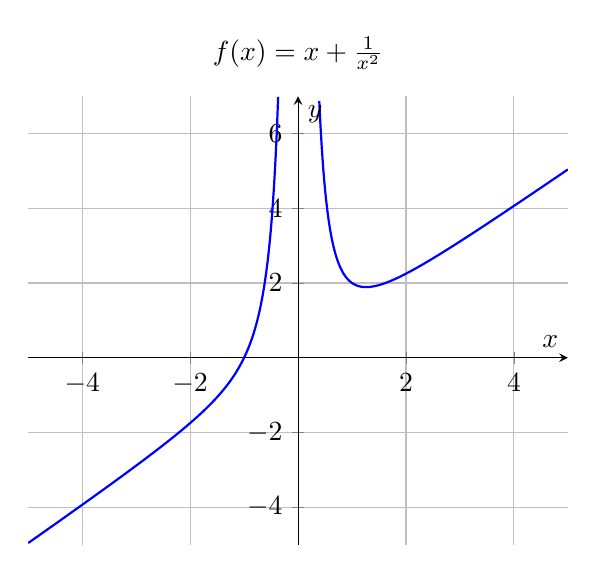
\begin{tikzpicture}
    \begin{axis}[
        title={$f(x) = x + \frac{1}{x^2}$},
        axis lines = middle,
        grid = major,
        xlabel={$x$},
        ylabel={$y$},
        xmin=-5, xmax=5,      % Ajusta la ventana en x
        ymin=-5, ymax=7,      % Ajusta la ventana en y
        restrict y to domain=-5:7, % Corta valores de y fuera de [-5,7]
        unbounded coords=jump, % Salta las discontinuidades en vez de trazar líneas infinitas
        samples=200
    ]
    % Dividimos el dominio en 2 intervalos para evitar x=0 (asíntota vertical)
    \addplot[domain=-5:-0.2, thick, blue] {x + 1/(x^2)};
    \addplot[domain=0.2:5, thick, blue] {x + 1/(x^2)};
    \end{axis}
\end{tikzpicture}